% Delete-min, pass 2: meld the resulting heaps from right to left.
% Editable source for this diagram. From this directory, regenerate with:
% latex -interaction=nonstopmode -halt-on-error pairing-heap-5.tex
% dvisvgm --no-fonts --exact --bbox=papersize --output=pairing-heap-5.svg pairing-heap-5.dvi
\documentclass[tikz,border=2pt]{standalone}
\usepackage{lmodern}
\usepackage{tikz}
\usetikzlibrary{arrows.meta,backgrounds,shapes.geometric,patterns}
\definecolor{linkred}{HTML}{B5240A}
\definecolor{noteBlue}{HTML}{0067A5}
\definecolor{softgreen}{HTML}{D8EAD0}
\definecolor{softpurple}{HTML}{D9D1E8}
\definecolor{softpink}{HTML}{F5CECF}
\definecolor{softyellow}{HTML}{FFF2C9}
\begin{document}
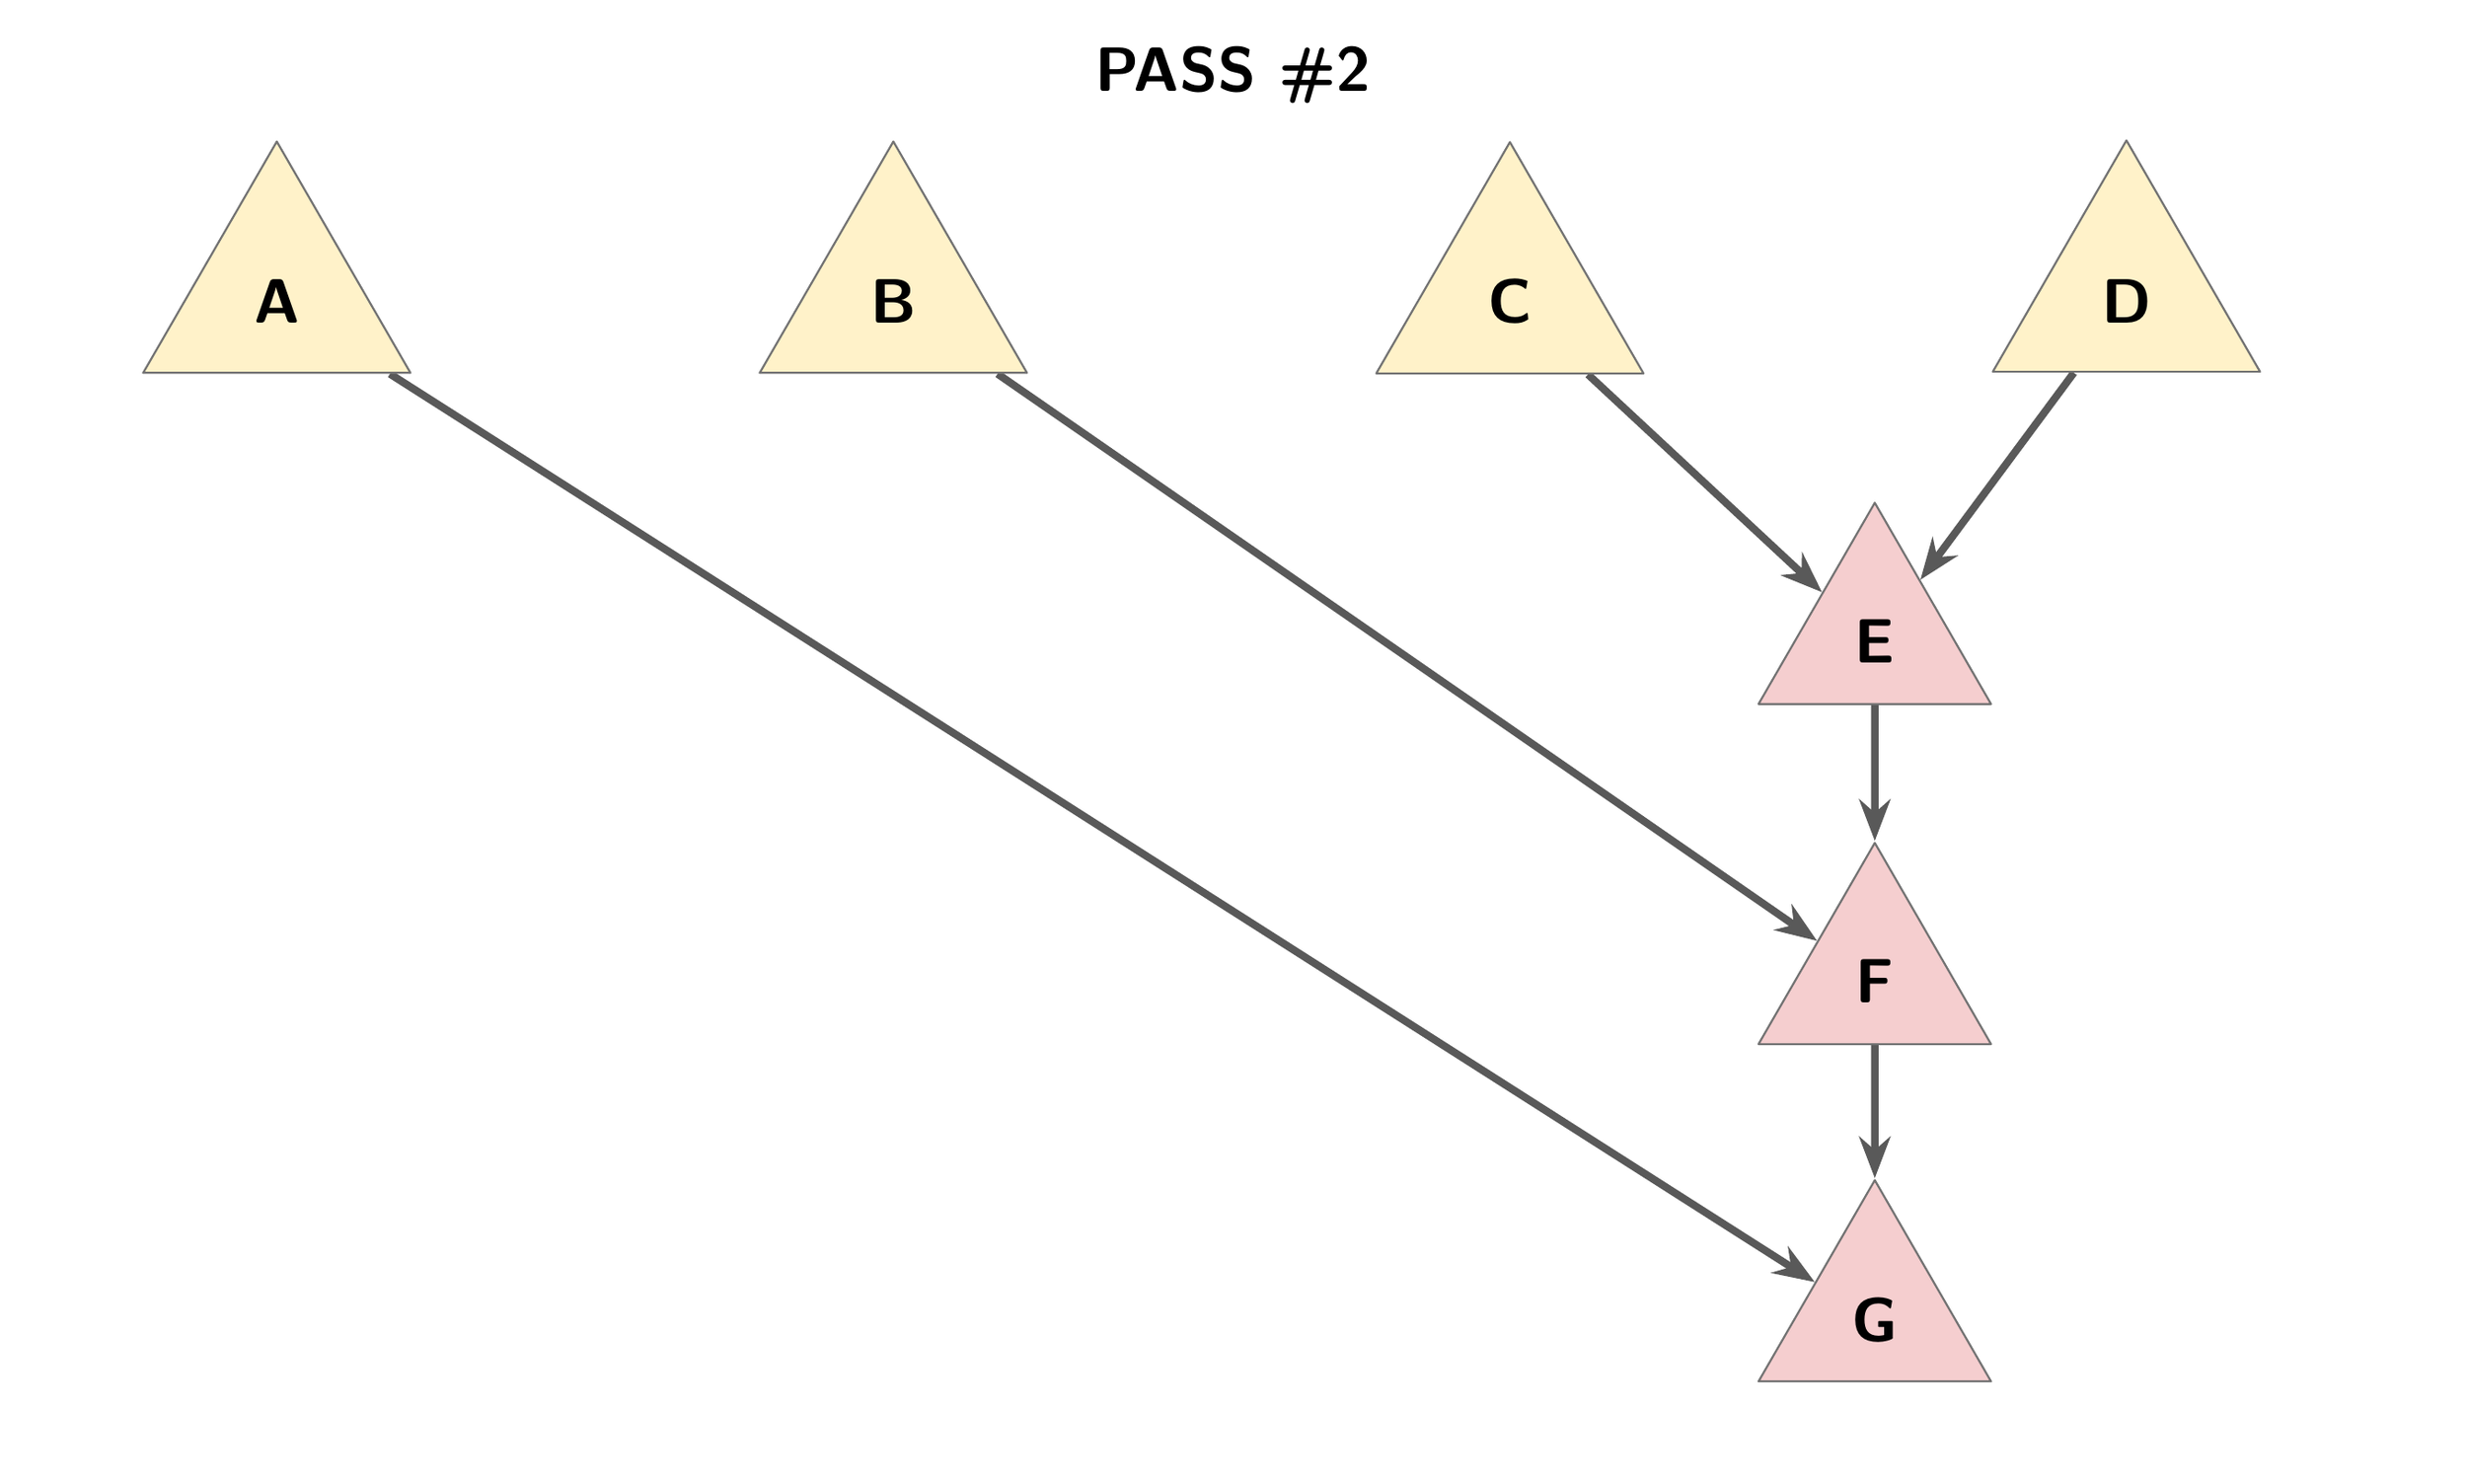
\begin{tikzpicture}[x=1pt,y=-1pt,>=Stealth,line cap=round,line join=round]
\path[use as bounding box] (0,0) rectangle (960,570);
\begin{scope}[on background layer]

\end{scope}
\node[isosceles triangle,draw=black!55,fill=softyellow,text=black,minimum size=92pt,inner sep=0pt,line width=0.8pt,font=\sffamily\fontsize{27}{32.4}\selectfont,shape border rotate=90,isosceles triangle apex angle=60,font=\sffamily\bfseries\fontsize{27}{32}\selectfont] (A) at (100,110) {A};
\node[isosceles triangle,draw=black!55,fill=softyellow,text=black,minimum size=92pt,inner sep=0pt,line width=0.8pt,font=\sffamily\fontsize{27}{32.4}\selectfont,shape border rotate=90,isosceles triangle apex angle=60,font=\sffamily\bfseries\fontsize{27}{32}\selectfont] (B) at (345,110) {B};
\node[isosceles triangle,draw=black!55,fill=softyellow,text=black,minimum size=92pt,inner sep=0pt,line width=0.8pt,font=\sffamily\fontsize{27}{32.4}\selectfont,shape border rotate=90,isosceles triangle apex angle=60,font=\sffamily\bfseries\fontsize{27}{32}\selectfont] (C) at (590,110) {C};
\node[isosceles triangle,draw=black!55,fill=softyellow,text=black,minimum size=92pt,inner sep=0pt,line width=0.8pt,font=\sffamily\fontsize{27}{32.4}\selectfont,shape border rotate=90,isosceles triangle apex angle=60,font=\sffamily\bfseries\fontsize{27}{32}\selectfont] (D) at (835,110) {D};
\node[isosceles triangle,draw=black!55,fill=softpink,text=black,minimum size=80pt,inner sep=0pt,line width=0.8pt,font=\sffamily\fontsize{27}{32.4}\selectfont,shape border rotate=90,isosceles triangle apex angle=60,font=\sffamily\bfseries\fontsize{27}{32}\selectfont] (E) at (735,245) {E};
\node[isosceles triangle,draw=black!55,fill=softpink,text=black,minimum size=80pt,inner sep=0pt,line width=0.8pt,font=\sffamily\fontsize{27}{32.4}\selectfont,shape border rotate=90,isosceles triangle apex angle=60,font=\sffamily\bfseries\fontsize{27}{32}\selectfont] (F) at (735,380) {F};
\node[isosceles triangle,draw=black!55,fill=softpink,text=black,minimum size=80pt,inner sep=0pt,line width=0.8pt,font=\sffamily\fontsize{27}{32.4}\selectfont,shape border rotate=90,isosceles triangle apex angle=60,font=\sffamily\bfseries\fontsize{27}{32}\selectfont] (G) at (735,515) {G};
\begin{scope}[on background layer]
\draw[draw=black!65,line width=3pt,->] (C) -- (E);
\draw[draw=black!65,line width=3pt,->] (D) -- (E);
\draw[draw=black!65,line width=3pt,->] (B) -- (F);
\draw[draw=black!65,line width=3pt,->] (E) -- (F);
\draw[draw=black!65,line width=3pt,->] (A) -- (G);
\draw[draw=black!65,line width=3pt,->] (F) -- (G);
\end{scope}
\node[anchor=center,text=black,font=\sffamily\fontsize{32}{38.4}\selectfont,font=\sffamily\bfseries\fontsize{32}{38}\selectfont] at (480,20) {PASS \#2};
\end{tikzpicture}
\end{document}
